




\section{Mapeamento}
Vamos começar a entender o que é uma estrutura algébrica como introdução. Tome um conjunto $S$ e incorpore esse conjunto com uma estrutura algébrica assumindo que nós podemos combinar, de várias formas (geralmente em duas), os elementos desse conjunto $S$ para obter os elementos desse conjunto $S$. Isso que estamos fazendo aqui é combinar elementos do conjunto $S$, denominado de \textit{operações em $S$}. Uma coisa importante para saber agora é que o comportamento dessas operações em $S$ podem ser condicionadas impondo certos axiomas, alterando a natureza de $S$. Os axiomas definem a particularidade da estrutura em $S$. Se eu quiser pegar uma coleção de axiomas e testá-los na tentativa de definir novas estruturas seria algo possível. Repare nas palavras "testá-los" e "tentativa". Uma estrutura algébrica depende fortemente de \textbf{consistência} entre sua coleção de axiomas. Mesmo assim ainda não seria suficiente para evitar criar um sistema estranho. Daqui em diante trataremos os axiomas como regras que são validadas dentro de um sistema algébrico, não como verdades evidentes como é popularmente entendido.
\subsection{Função Geral}
Sendo $S$ um conjunto de todos os objetos em venda num mercado e $T$ ser o conjunto de todos os números reais. Definimos $f:S \to T$ como $f(s) = \textrm{preço de s}$. Isso é um exemplo de mapeamento de $S$ para $T$.
Um exemplo de função: Sendo $S$ um conjunto não vazio e definindo $i:S \to S$ como $i(s) = s$ para qualquer $s \in S$. Chamamos essa função, onde temos $S$ para $S$, de função identidade.\newline
Um mapeamento é uma função geral que associa um elemento de uma origem a um elemento \textbf{único} do destino. Chamaremos $f$ como um mapeamento de $S$ para $T$ por $f:S \to T$ e, para $t \in T$, $t = f(s)$; $t$ é \textit{imagem} de $s$ sob $f$.
Assim, uma função é um mapa de um domínio $D$ para um contradomínio $CD$ tal que cada elemento de $D$ tem pelo menos uma imagem em $CD$.

\begin{definition}
  Se $g:S \to T$ e $f:T \to U$, então a \emph{composição}, denotada por $f \circ g$, é o mapameanto $f \circ g: S \to U$ definido por $(f \circ g)(s) = f(g(s))$ para todo $s \in S$.
\end{definition}
\begin{lemma}\label{comp-assoc}
  Se $h:S \to T, g:T \to U$\ e\ $f:U \to V$, então $f\circ (g\circ h) = (f \circ g)\circ h.$
  \begin{proof}
    Temos que verificar que se esses dois mapeamento são iguais eles devem fazer a mesma coisa para qualquer elemento.\\
    $\forall s \in S, (f\circ(g\circ h))(s) = ((f \circ g)\circ h)(s).$ A aplicação da definição de composição segue $$(f\circ (g\circ h))(s)=f((g\circ h)(s))=f(g(h(s)))$$ $$((f\circ g)\circ h)(s)=(f\circ g)(h(s))=f(g(h(s))),$$ $$(f\circ (g \circ h))(s)=((f \circ g)\circ h)(s), \forall s \in S.$$
    Consequentemente, por definição, $f \circ (g \circ h) = (f\circ g) \circ h.$
  \end{proof}
\end{lemma}

\subsubsection{Funções Lineares}
Uma das mais importantes classes de funções. Considere o conjunto 
$$ \R_{m}^{n} = \left\{
  \begin{bmatrix}
    a_{11} & \cdots & a_{1n} \\
    \vdots &  & \vdots \\
    a_{m1} & \cdots & a_{mn}
  \end{bmatrix}
\mid a_{ij} \in \R \right\}.$$
Em particular, $\R_{2}^{1}$ é o conjunto dos vetores coluna bidimensionais 
$$\hat{v} = \begin{bmatrix}
  v_{1} \\
  v_{2}
\end{bmatrix}; v_{1}, v_{2} \in \R.$$
Cada matriz real quadrada de ordem $2$ resulta em uma função linear
$$ L_{A}:\R_{2}^{1} \to \R_{2}^{1}; \begin{bmatrix}
  v_{1} \\
  v_{2}
\end{bmatrix}
\mapsto 
\begin{bmatrix}
  a_{11}v_{1} + a_{12}v_{2} \\
  a_{21}v_{1} + a_{22}v_{2}
\end{bmatrix}$$
ou $$L_{A}\left(\hat{v}\right) = A\hat{v}.$$
Claro que $$L_{A} \begin{bmatrix}
  1 \\
  0
\end{bmatrix} =
\begin{bmatrix}
  a_{11} \\
  a_{21}
\end{bmatrix} \quad \textrm{e} \quad
L_{A} \begin{bmatrix}
  0 \\
  1
\end{bmatrix} =
\begin{bmatrix}
  a_{12} \\
  a_{22}
\end{bmatrix},$$
isto é, a função linear $L_{A}$ determina a matriz $A$.

Seja $B$ uma matriz quadrada de ordem $2$ com uma função linear correspondente $L_{B}: \hat{v}\mapsto B\hat{v}$, $BA$ é definida por
$$\begin{bmatrix}
  b_{11} & b_{12} \\
  b_{21} & b_{22}
\end{bmatrix}
\begin{bmatrix}
  a_{11} & a_{12} \\
  a_{21} & a_{22}
\end{bmatrix} = 
\begin{bmatrix}
  b_{11}a_{11} + b_{12}a_{21} + b_{12}a_{22} \\
  b_{21}a_{11} + b_{22}a_{21} + b_{22}a_{22}
\end{bmatrix}.$$
A equação $L_{BA} (\hat{v}) = L_{B} \circ L_{A} (\hat{v})$ é verdadeira para todo $\hat{v}$ em $\R_{2}^{1}$. 

A multiplicação de matrizes acompanha a composição das funções lineares correspondentes. Em particular, a associatividade da multiplicação de matriz é uma consequência direta da associatividade da composição de funções (\textbf{Lema} \ref{comp-assoc}).

\subsubsection{Semigrupos de Funções}
Um mapa (ou função) $f: X \to X$ de $X$ para ele mesmo é muitas vezes dito como um \emph{autom-mapa} do conjunto $X$. Nesse contexto, o conjunto algumas vezes é chamado de \emph{conjunto base} para a função $f: X \to X$.
\begin{definition}
  Um conjunto $S$ de funções $f: X \to X$ com o domínio $X$ e contradomínio $X$ é dito ser um semigrupo de funções no conjunto base $X$ se $$f\quad \textrm{e}\quad g\quad \textrm{em}\quad S\quad \textrm{implica}\quad g \circ f\quad \textrm{em}\quad S. $$
Nesse caso, $S$ está fechado sob a composição (composta).

Se $f$ é um elemento de um semigrupo $S$ de funções, as exponenciais $f^n$ para $n$ inteiros positivos são definidas recursivamente por $f^{1} = f$ e $f^{n+1} = f^n \circ f.$

Alguns exemplos de semigrupos de funções são:
\begin{exmp}[Auto-mapas]
  Para um conjunto base $X$, defina $X^X$ como o conjunto de todas as funções de $X$ para $X$. Então $X^X$ forma um semigrupo de funções em $X$.
\end{exmp}
\end{definition}
\begin{exmp}[Funções constantes]
  Seja $X$ um conjunto e $Y$ um subconjunto de $X$. Para cada elemento $y$ de $Y$, define uma função constante
  \begin{alignat}{2}
    c_{y}:\ &X \to X \nonumber\\
    &x\ \mapsto\ y.
    \nonumber
  \end{alignat}
  Ainda temos que para cada elemento $x$ de $X$, $y \in X$ e $z$ no subconjunto $Y$
  $$c_{z} \circ c_{y}(x) = c_{z}\left(c_{y}(x)\right) = c_{z}(y) = z = c_{z}(x),$$
  ou seja, $c_{z} \circ c_{y} = c_{z}$. Assim o conjunto $$C_{Y} = \left\{c_{y}\mid y \in Y\right\}$$ forma um semigrupo de funções em $X$.
\end{exmp}
\begin{definition}[Função identidade]
  Para qualquer conjunto $X$, a função identidade $id_{X}$ é definida por
  \begin{alignat}{2}
    id_{X}:\ &X \to X \nonumber\\
    &x\ \mapsto\ x.
    \nonumber
  \end{alignat}
  Para conjuntos $X$, $Y$ e $f: X \to Y$, temos
  $$id_{Y}\circ f = f = f \circ id_{X}.$$
\end{definition}
\begin{definition}[Monóide de Funções]
  Um conjunto $S$ de auto-mapas em um conjunto base $X$ é dito ser um monóide de funções em $X$ se formar um semigrupo e se a função identidade $id_{X}$ é um elemento de $S$.
\end{definition}
Um exemplo trivial de um monóide de função é o conjunto $X^X$ em $X$.
\begin{exmp}
Pelas funções lineares o conjunto $L\left(2,\R\right)$ das funções lineares de $\R_{2}^{1}$ para ele mesmo forma um semigrupo de funções em $\R_{2}^{1}$. Agora para a matriz identidade
$$I_{2} = \begin{bmatrix}
    1 & 0\\
    0 & 1
  \end{bmatrix}
$$
a função linear $L_{I_{2}}$ é a função identidade $id_{\R_{2}^{1}}$, então $L\left(2,\R\right)$ forma um monóide de funções em $\R_{2}^{1}.$
\end{exmp}

\subsubsection{Injetividade e sobrejetividade}
Um mapeamento (a função $f$) $f: X \to Y$ precisa associar um unico valor da função $f(x)$ no contradomínio $Y$ para cada argumento $x$ do domínio $X$. Por outro lado, pode acontecer que argumento diferentes sejam associados ao mesmo valor $f(x)$. O caso trivial que serve de exemplo é a função dos quadrados $sq: \Z \to \N$ onde poderiamos ter $$sq(-5) = (-5)^{2} = 25 = 5^{2} = sq(5).$$
\begin{definition}[Função Injetiva]
	Uma função $f: X \to Y$ é dita ser injetiva, ou \emph{um para um}, se $$f(x) = f(x') \implies x = x'$$
  para todos elementos $x$ e $x'$ do domínio $S$.
  Em essência, a equação $f(s) = t$ precisa ter uma única solução $x$ em $X$ para cada elemento $y$ para a imagem de $f$. É imediato que qualquer função com um domínio vazio seja injetiva. Diferente da função $sq: \Z \to N$, a função $sqn: \N \to \N; n \mapsto n^{2}$ é injetiva.
\end{definition}
\begin{stat}[Retração de funções injetivas]
  Deixe $f: X \to Y$ injetiva, com o domínio não vazio. Então existe uma função $$r: Y \to X$$
  tal que $$r \circ f = id_{X}.$$
\end{stat}
\begin{proof}
  Escolha um elemento $x_{0}$ de $X$. Para um elemento $y$ do contradomínio que
  não está na imagem $f(X)$, defina $r(y) = x_{0}$. Agora considere um elemento $y$ da imagem de $f(X)$. Pela definição de imagem, a equação $f(x) = y$ tem um solução. Como $f$ é injetiva, a solução é única. 
  
  Defina $r(y)$ como este único elemento de solução $x_{y}$. 
  
  Obtemos uma função $r: Y \to X$. Agora $r \circ f: X \to X$. Então para cada elemento $x$ de $X$, temos $$r\circ f(x) = r \left(f(x)\right) = x_{f(x)} = x = id_{X}(x),$$ que verifica $r \circ f = id_{X}.$
\end{proof}
\begin{definition}[Retração]
  Um mapeamento $r: Y \to X$ é cahamado de uma retração de uma função $f: X \to Y$ se $r\circ f = id_{X}.$
\end{definition}
\begin{stat}[Funções com retrações são injetivas]
  Se uma função $f: X \to Y$ possui uma retração (volta), então ela é injetiva.
\end{stat}
\begin{proof}
  Deixe $r: Y \to X$ ser uma retração para $f$. Então $$f(x) = f(x') \implies x=r\circ f(x) = r\circ f(x') = x'$$ para $x,x'$ em $X$.
\end{proof}
A proprosição anterior mostra que cada injeção com domínio não vazio tem uma retração. Note que um injeção $f$ pode ter muitas retrações, por causa da escolha arbitrária do elemento $x_{0}$ na prova da existência da retração. Também, note que a função identidade $id_{\varnothing}$ no conjunto vazio possui sua própria retração.


\begin{definition}[Função Sobrejetiva]
	Uma função $f: X \to Y$ é dita ser sobrejetiva se o contradomínio e imagem coincidem: $Y = f(X)$.
\end{definition}
Maneiras para dizer que um mapeamento $f: X \to Y$ é sobrejetivo:
$$f(X) = \{f(x) \in Y \mid x \in X\}$$
$$f(X) = Y.$$
Ainda, a imagem inversa $$f^{-1}\{y\} = \left\{x \in X \mid f(x) = y\right\}$$
necessita ser não vazia para cada elemento $y$ de $Y$. Perceba que a única função sobrejetiva com um domínio vazio é a função identidade $id_{\varnothing}$ no conjunto vazio.

Um exemplo trivial de uma função sobrejetiva seria a função do valor absoluto $abs: \Z \to \N; n \mapsto \mid n \mid$
\begin{stat}[Seções de funções sobrejetivas]
  Deixe $f: X \to Y$ ser sobrejetiva. Então existe uma função $$s: Y \to X$$ tal que $$f \circ s = id_{y}.$$
\end{stat}
\begin{definition}[Seções]
  Uma função $s: Y \to X$ é chamada de seção de uma função $f: X \to Y$ se $f \circ s = id_{Y}.$
\end{definition}
\begin{stat}[Funções com seções são sobrejetivas]
  Se uma função $f: X \to Y$ tem uma seção, então ela é sobrejtiva.
  \begin{proof}
    Deixe $s: Y\to X$ ser uma seção para $f$. Então $$f\left(s(y)\right) = f\circ s(y) = id_{Y} = y$$
    para cada elemento $y$ de $Y$.
  \end{proof}
\end{stat}
Cada sobrejeção tem uma seção. Note que uma sobrejeção $f$ pode ter muitas seções.

\subsubsection{Isomorfismo}
\begin{definition}[Isomorfismo de conjuntos]
    A função $f:X \to Y$ é bijetivo se $f$ é injetivo e sobrejetivo.
\end{definition}
A utilização do mapeamento começa a se expandir quando entramos em composições de mapeamentos. Situa-se dois mapeamentos $g:X \to Y$ e $f:Y \to Z$. Queremos fazer com que os elementos de $X$ sejam conduzidos ao conjunto $Z$. Com efeito, $g(x) \in Y$, sendo $f:Y \to Z$, tem-se a disponibilidade de $f(g(x)) \in Z$. Assim, $(f\circ g):X \to Z$. Então, há o mapeamento de $X$ para $Z$.
\begin{lemma}
  Se $f:X \to Y$ é uma bijeção, então $f\circ f^{-1} = id_{Y}$ e $f^{-1} \circ f=id_{X}$, onde $id_{X}$ e $id_{Y}$ são as identidades dos mapeamentos de $X$ e de $Y$, respectivamente.
  \begin{proof}
    Primeiramente, temos $(f\circ f^{-1})(y)=f(f^{-1}(y))$. Pela definição, $f^{-1}$ é o elemento $x_{0}\in X$ tal que $y=f(x_{0})$. Então $f(f^{-1}(y))=f(x_{0})=y$. Ora, isso significa que $(f\circ f^{-1})(y) = y$, validando a identidade deste mapeamento em $Y$.
  \end{proof}
\end{lemma}
Para $f^{-1}\circ f = id_{X}$ funciona analogamento como para $id_{Y}$
\begin{definition}
  Para uma função $f: X \to Y$, uma função $g: Y \to X$ satisfazendo $g \circ f = id_{x}$ e $f \circ g = id_{Y}$ é chamado de inversa de $f$.
\end{definition}
Se existe um isomorfismo $f: X \to Y$ de um conjunto $X$ para um conjunto $Y$, podemos escrever $$X \cong Y$$ e dizer que os conjunto $X$ e $Y$ são isomorfico. Nesse caso $Y \cong X$, em virtude do isomorfismo $f^{-1}$. 

A ténica padrão para mostrar que dois conjuntos $X$ e $Y$ são isomorficos exibir duas funções mutuamente inversas $f: X \to Y$ e $g: Y \to X$.

\begin{exmp}
  Para cada númera natural $n$, considere o conjunto finito $$N = \{0,1,2, ..., n -1\}$$
  dos números naturais menos do que $n$. Note que o conjunto $N$ tem $n$ elementos. Em particular, $\widehat{0}$ é o conjunto vazio. Agora, se um conjunto finito $X$ tem $n$ elementos, digamos $X = \{x_{0},x_{1},...,x_{n-1}\}$, então existe uma bijeção
  \begin{alignat}{2}
    K:\ &N \to X \nonumber\\
    &i\ \mapsto\ x_{i}.
    \nonumber
  \end{alignat}
\end{exmp}
De fato, um conjunto $X$ tem $n$ elementos se, e somente se existe uma bijeção $K: N\to X$. Nós podemos dizer que $K$ \emph{conta}  os elementos de $X$. O número dos elemetnos em um conjunto finito $X$ é chamado de \emph{tamanho} ou \emph{ordem} de $X$. É escrito como $\mid X\mid$. Dois conjunto são isomorficos se e somente se $\mid X\mid = \mid Y\mid$.

\subsubsection{Grupos de permutações}
\begin{definition}
  Deixe $X$ ser um conjunto.
  \begin{enumerate}(i.)
    \item Uma função bijetiva $f: X \to X$ é chamada de uma permutação do conjunto $X$.
    \item Um conjunto $G$ de permutações em $X$ é dito ser um grupo de permutações de $X$ ou uma permutação no conjunto $X$ se $G$ é um monóide de funções satisfazendo a seguinte propriedade $$f \in G \implies f^{-1} \in G$$, também conhecida como \emph{fechada sob a inversão}.
  \end{enumerate}
\end{definition}

\subsection{Equivalência}
Ao estudarmos uma estrutura precisamos filtrar o que não é relevante para o estudo dela. A equivalência é este filtro. Um exemplo inicial de sua necessidade surge no conceito de número. O que significa o número 3? Um conjunto $X$ tem 3 elementos se e somente se existe um isomorfismo de conjunto $$f: \{1,2,3\} \to X$$
contando os elementos de $X$ como $f(1), f(2)$ e $f(3)$. A função $f$ tem que ser injetiva, de modo que nenhum elemento de $X$ seja contado duas vezes. A função $f$ tem que ser sobrejetiva, para garantir que cada elemento de $X$ seja contado.

O único problema aqui é a circularidade. Para caracterizar o número 3, nós usamos esse número no domínio da função acima. Para escapar da circularidade nós podemos decidir considerar dois conjuntos como equivalentes para própositos de contagem sempre que eles forem isomórficos. O número 3 surge então como a propriedade que é comum a cada um dos conjuntos que são isomórficos a algum dado conjunto de 3 elementos (por exemplo $\{1,2,3\})$ ou $\{\varnothing , \{\varnothing\} , \{\{\varnothing\}\}\}$). Os detalhes particulares dos elementos nos conjuntos não são relevantes para o problema da contagem, Eles são filtrados pela equivalência.

\subsubsection{Núcleo e relações de equivalência}
Considere a função dos quadrados $sq: \Z \to \Z; n\mapsto n^{2}$. Para dois inteiros $n_{1}$ e $n_{2}$, $$sq(n_{1}) = sq(n_{2})\quad \textrm{iff}\quad n_{2} = \pm n_{1}.$$
Isto é, os inteiros $n_{1}$ e $n_{2}$ são associados ao mesmo valor de saída (valor da função) se e somente se ambos estão na mesma classe de equivalência $\{r, -r\}$. Essas classes de equivalência dividem o conjunto de domínios $\Z$ de inteiros, o que significa que $\Z$ se decompõe como a união 
$$ \Z = \{0\} \cup \{\pm 1\} \cup \{\pm 2\} \cup \{\pm 3\} \cup ...$$
de subconjuntos mutuamente disjuntos, as classes de equivalências.
\begin{definition}[Relação de núcleo(kernel) de uma função]
  Considere uma função $f: X \to Y$. Um par $\langle x{1}, x{2} \rangle$ de elementos de $X$ é dito estar na relação de núcleo $ker\ f$, denotada por $x{1} ker\ f x{2}$ ou por $x{1} (ker\ f) x{2}$, se e somente se $x{1}$ e $x{2}$ são associados com a mesma saída (valor da função) por $f$. Formalmente
  $$ x{1} (ker\ f) x{2}\quad \textrm{iff}\quad f(x{1}) = f(x{2}).$$
\end{definition}
A relação de núcleo $ker f$ de uma função $f: X \to Y$ é reflexiva: $$ x (ker f) x$$ para todo $x$ em $X$. Também é transitiva: $$\left(x_{1} (ker f) x_{2}\quad \textrm{e}\quad x_{2} (ker f) x_{3}\right) \implies x_{1} (ker f) x_{3},$$ como $f(x_{1}) = f(x_{2})$ e $f(x_{2}) = f(x_{3})$ implica em $f(x_{1}) = f(x_{3}).$ E, por fim, também é simétrica: $$ x_{1} (ker f) x_{2} \implies x_{2} (ker f) x_{1}.$$
\begin{stat}[Núcleos são relações de equivalência]
  Deixe $f: X \to Y$ ser uma função. Então a relação de núcleo $ker f$ de $f$ é uma relação de equivalência no domínio $X$ da função $f$.
\end{stat}

\subsubsection{Classes de equivalência}
O kernel da função quadrática $sq: \Z \to \Z$ produziu a partição $ \Z = \{0\} \cup \{\pm 1\} \cup \{\pm 2\} \cup \{\pm 3\} \cup ...$ de $\Z$. Temos que cada relação de equivalência em um conjunto produz uma partição do conjunto.

\begin{definition}
  Se $R$ é uma relação de equivalência em um conjunto $X$, define a classe de equivalência de $x$ sob $R$ sendo o conjunto $$ \left[x\right]_{R} = \left\{t \in X \mid x R t\right\}$$ de todos os elementos $t$ de $X$ que estão relacionados a $x$ por $R$.
\end{definition}
Pela reflexividade cada classe $\left[x\right]_{R}$ é não vazia porque contém pelo menos o próprio $x$. Pela relação kernel (ker $f$) de uma função $f: X\to Y$, e para um elemento $x$ do domínio $X$, as classes de equivalência são dados pelos conjuntos de imagem inversa $$\left[x\right]_{ker\ f} = f^{-1}\{f(x)\}.$$ Aqui está a propriedade chave de particionamento das relações de equivalência.

\begin{stat}[Classes de equivalência são disjuntas ou iguais]\label{PropLag1}
  Deixe $R$ ser uma relação de equivalência no conjunto $X$. Deixe $x_{1}$ e $x_{2}$ serem elementos de $X$. Então as duas classes equivalência $\left[x_{1}\right]_{R}$, $\left[x_{2}\right]_{R}$ são ambas disjuntas: $$\left[x_{1}\right]_{R} \cap \left[x_{2}\right]_{R} = \varnothing$$ ou iguais $$\left[x_{1}\right]_{R} = \left[x_{2}\right]_{R}.$$ Em último caso, $x_{1} R x_{2}$.
  \begin{proof}
    Suponha que $\left[x_{1}\right]_{R}$ e $\left[x_{2}\right]_{R}$ não são disjuntos. Assim, eles possuem um elemento $x'$ em comum. Então $x_{1} R x'$ e $x_{2} R x'$ pela definição de classes de equivalência. Pela \emph{simetria}, $x' R x_{2}$. Então $x_{1} R x'$ e $x' R x_{2}$ implica em $x_{1} R x_{2}$ pela \emph{transitividade}.

    Suponha que $x''$ é um elemento de $\left[x_{1}\right]_{R}$, então $x_{1} R x''$. Então $$ x_{2} R x_{1} R x''$$ implica $x_{2} R x''$ pela transitividade, assim $x''$ é um elemento de $\left[x_{2}\right]_{R}$. Similarmente, cada elemento de $\left[x_{2}\right]_{R}$ é um elemento de $\left[x_{1}\right]_{R}$. Segue que as duas classes $\left[x_{1}\right]_{R}$ e $\left[x_{2}\right]_{R}$ são iguais.
  \end{proof}
\end{stat}
Concluindo, temos que cada relação de equivalência $R$ no conjunto $X$ é a relação kernel de uma função adequada com $X$ como domínio. Deixe $X_{R}$ denotar o conjunto $$\{\left[x\right]_{R} \mid x \in X\}$$ de todas as classes de equivalência sob $R$. É muito importante observar que $X_{R}$ é um conjunto de conjuntos. Os elementos $C$ do conjunto $X_{R}$ são conjuntos (as classes de equivalências). É importante este conceito final porque está presente em uma das principais dificuldades no entendimento da algebra. A hierarquia (elementos - conjuntos - conjuntos de conjuntos) deve ser compreendida o mais breve possível antes de chegarmos a uma abstração mais avançada.

\begin{stat}
  Deixe $R$ ser uma relação de equivalência em um conjunto $X$.
  \begin{enumerate}[(a)]
    \item Existe uma função sobrejetiva $$nR: X\to X_{R};\ x\mapsto \left[x\right]_{R}.$$
    \item A relação de núcleo da função $nR$ é o próprio $R$.
  \end{enumerate}
\end{stat}
\newpage

\subsubsection{O primeiro Teorema de Isomorfismo para conjuntos}
A função de divisão $\setminus: X\to \R; (n,m) \mapsto n^{-1}m$ (sendo a imagem dessa função o conjunto dos racionais) se decompõe como um composto da sobrejeção $X \to X_{R}$, o isomorfismo $X_{R} \cong \Q$, e a injeção $\Q \hookrightarrow \R$. O primeiro Teorema de Isomorfismo para conjuntos mostra que toda função pode ser escrita como uma composição $$\langle \textrm{injeção} \rangle \circ \langle \textrm{isomorfismo} \rangle \circ \langle \textrm{sobrejeção} \rangle $$
\begin{mymdframed}{Notação}
  $\hookrightarrow$ denota um monomorfismo, ou morfismo injetivo. Como $\Q \subset \R$ , isto é, neste contexto, $\Q$ é uma subestrutura de $\R$, temos uma injeção natural, onde os elementos de $\Q$ são tratados como um elemento de $\R$.
\end{mymdframed}
Considere uma função $f: X\to Y$. Como a relação de núcleo $ker\ f$ é uma relação de equivalência, a proposição (a) anterior mostra que existe uma função sobrejetiva $$s: X\to X_{ker\ f};\ x\mapsto \left[x\right]_{ker\ f}.$$
Por outro lado, existe uma injeção $$j: f(X) \hookrightarrow Y;\ y\mapsto y$$ inserindo a imagem $f(X)$ como um subconjunto no contradomínio $Y$.
O ingrediente restante é um isomorfismo entre o conjunto $X_{ker\ f}$ das classes de núcleo e a imagem $f(X)$.

\begin{stat}
  Deixe $f: X\to Y$ ser uma função. Então existe uma \emph{bijeção bem definida} $$ b: X_{ker\ f} \to f(X);\ \left[x\right]_{ker\ f} \mapsto f(x).$$
\end{stat}
\begin{theorem}[Primeiro Teorema de Isomorfismo para conjuntos]
  Deixe $f: X\to Y$ ser uma função. Então $f$ se decompõe como a composta $$f = j\circ b \circ s.$$ 
\end{theorem}

\begin{center}
\tikzset{every picture/.style={line width=0.75pt}} %set default line width to 0.75pt
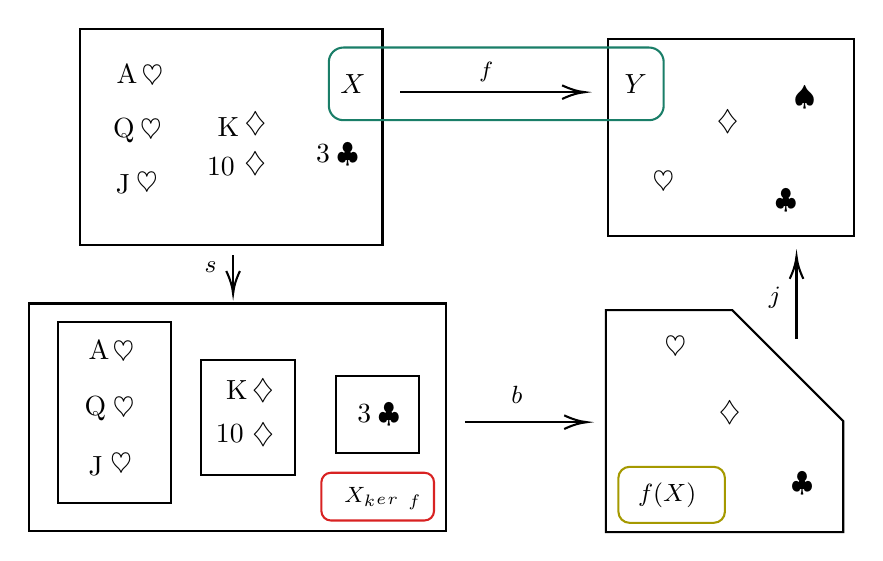
\begin{tikzpicture}[x=0.75pt,y=0.75pt,yscale=-1,xscale=1]
%uncomment if require: \path (0,283); %set diagram left start at 0, and has height of 283

%Shape: Rectangle [id:dp706505862263574] 
\draw   (136.2,20.93) -- (281.87,20.93) -- (281.87,124.93) -- (136.2,124.93) -- cycle ;
%Straight Lines [id:da3693556638631299] 
\draw    (209.87,130.07) -- (209.87,146.6) ;
\draw [shift={(209.87,148.6)}, rotate = 270] [color={rgb, 255:red, 0; green, 0; blue, 0 }  ][line width=0.75]    (10.93,-3.29) .. controls (6.95,-1.4) and (3.31,-0.3) .. (0,0) .. controls (3.31,0.3) and (6.95,1.4) .. (10.93,3.29)   ;
%Shape: Rectangle [id:dp04842635536868545] 
\draw   (111.4,153.33) -- (312.27,153.33) -- (312.27,262.87) -- (111.4,262.87) -- cycle ;
%Shape: Rectangle [id:dp4296555353151592] 
\draw   (125.6,162.07) -- (179.87,162.07) -- (179.87,249.27) -- (125.6,249.27) -- cycle ;
%Shape: Rectangle [id:dp10721044735746443] 
\draw   (194.4,180.47) -- (239.87,180.47) -- (239.87,236.07) -- (194.4,236.07) -- cycle ;
%Shape: Rectangle [id:dp05111312242076149] 
\draw   (259.6,188.47) -- (299.47,188.47) -- (299.47,225.27) -- (259.6,225.27) -- cycle ;
%Rounded Rect [id:dp10074530866221898] 
\draw  [color={rgb, 255:red, 216; green, 34; blue, 34 }  ,draw opacity=1 ] (252.4,239.47) .. controls (252.4,236.93) and (254.46,234.87) .. (257,234.87) -- (302.07,234.87) .. controls (304.61,234.87) and (306.67,236.93) .. (306.67,239.47) -- (306.67,253.27) .. controls (306.67,255.81) and (304.61,257.87) .. (302.07,257.87) -- (257,257.87) .. controls (254.46,257.87) and (252.4,255.81) .. (252.4,253.27) -- cycle ;
%Straight Lines [id:da9478383111897926] 
\draw    (321.5,210.5) -- (378.33,210.5) ;
\draw [shift={(380.33,210.5)}, rotate = 180] [color={rgb, 255:red, 0; green, 0; blue, 0 }  ][line width=0.75]    (10.93,-3.29) .. controls (6.95,-1.4) and (3.31,-0.3) .. (0,0) .. controls (3.31,0.3) and (6.95,1.4) .. (10.93,3.29)   ;
%Snip Single Corner Rect [id:dp578989805840413] 
\draw   (389.5,156.5) -- (450.33,156.5) -- (503.83,210) -- (503.83,263.5) -- (389.5,263.5) -- cycle ;
%Rounded Rect [id:dp27487588222286563] 
\draw  [color={rgb, 255:red, 165; green, 153; blue, 0 }  ,draw opacity=1 ] (395.5,237.4) .. controls (395.5,234.42) and (397.92,232) .. (400.9,232) -- (441.43,232) .. controls (444.42,232) and (446.83,234.42) .. (446.83,237.4) -- (446.83,253.6) .. controls (446.83,256.58) and (444.42,259) .. (441.43,259) -- (400.9,259) .. controls (397.92,259) and (395.5,256.58) .. (395.5,253.6) -- cycle ;
%Straight Lines [id:da08328439599003512] 
\draw    (481.33,170.5) -- (481.33,132.5) ;
\draw [shift={(481.33,130.5)}, rotate = 90] [color={rgb, 255:red, 0; green, 0; blue, 0 }  ][line width=0.75]    (10.93,-3.29) .. controls (6.95,-1.4) and (3.31,-0.3) .. (0,0) .. controls (3.31,0.3) and (6.95,1.4) .. (10.93,3.29)   ;
%Shape: Rectangle [id:dp9272690052599577] 
\draw   (390.5,26) -- (508.83,26) -- (508.83,121) -- (390.5,121) -- cycle ;
%Rounded Rect [id:dp384981296655891] 
\draw  [color={rgb, 255:red, 26; green, 126; blue, 104 }  ,draw opacity=1 ] (256,37) .. controls (256,33.13) and (259.13,30) .. (263,30) -- (410.33,30) .. controls (414.2,30) and (417.33,33.13) .. (417.33,37) -- (417.33,58) .. controls (417.33,61.87) and (414.2,65) .. (410.33,65) -- (263,65) .. controls (259.13,65) and (256,61.87) .. (256,58) -- cycle ;
%Straight Lines [id:da6106767055811906] 
\draw    (290.33,51.5) -- (377.33,51.5) ;
\draw [shift={(379.33,51.5)}, rotate = 180] [color={rgb, 255:red, 0; green, 0; blue, 0 }  ][line width=0.75]    (10.93,-3.29) .. controls (6.95,-1.4) and (3.31,-0.3) .. (0,0) .. controls (3.31,0.3) and (6.95,1.4) .. (10.93,3.29)   ;
\draw (151.93,89.87) node [anchor=north west][inner sep=0.75pt]   [align=left] {J};
\draw (161.6,88.6) node [anchor=north west][inner sep=0.75pt]    {$\heartsuit $};
\draw (150.6,62.53) node [anchor=north west][inner sep=0.75pt]   [align=left] {Q};
\draw (163.6,62.93) node [anchor=north west][inner sep=0.75pt]    {$\heartsuit $};
\draw (152.27,36.87) node [anchor=north west][inner sep=0.75pt]   [align=left] {A};
\draw (164.27,37.27) node [anchor=north west][inner sep=0.75pt]    {$\heartsuit $};
\draw (195.8,81.67) node [anchor=north west][inner sep=0.75pt]   [align=left] {10};
\draw (213.8,79.07) node [anchor=north west][inner sep=0.75pt]    {$\diamondsuit $};
\draw (200.87,62.4) node [anchor=north west][inner sep=0.75pt]   [align=left] {K};
\draw (213.87,59.8) node [anchor=north west][inner sep=0.75pt]    {$\diamondsuit $};
\draw (248.33,75.33) node [anchor=north west][inner sep=0.75pt]   [align=left] {3};
\draw (258.33,74.73) node [anchor=north west][inner sep=0.75pt]    {$\clubsuit $};
\draw (194.6,131.6) node [anchor=north west][inner sep=0.75pt]  [font=\small]  {$s$};
\draw (138.75,225.36) node [anchor=north west][inner sep=0.75pt]   [align=left] {J};
\draw (149.27,223.98) node [anchor=north west][inner sep=0.75pt]    {$\heartsuit $};
\draw (136.86,196.57) node [anchor=north west][inner sep=0.75pt]   [align=left] {Q};
\draw (150.4,196.95) node [anchor=north west][inner sep=0.75pt]    {$\heartsuit $};
\draw (138.78,169.54) node [anchor=north west][inner sep=0.75pt]   [align=left] {A};
\draw (150.32,169.91) node [anchor=north west][inner sep=0.75pt]    {$\heartsuit $};
\draw (200.13,210.4) node [anchor=north west][inner sep=0.75pt]   [align=left] {10};
\draw (217.63,209.62) node [anchor=north west][inner sep=0.75pt]    {$\diamondsuit $};
\draw (205.04,189.06) node [anchor=north west][inner sep=0.75pt]   [align=left] {K};
\draw (217.58,188.27) node [anchor=north west][inner sep=0.75pt]    {$\diamondsuit $};
\draw (268.3,200.57) node [anchor=north west][inner sep=0.75pt]   [align=left] {3};
\draw (278.28,199.84) node [anchor=north west][inner sep=0.75pt]    {$\clubsuit $};
\draw (262,240.27) node [anchor=north west][inner sep=0.75pt]  [font=\footnotesize]  {$X_{k}{}_{e}{}_{r}{}_{\ }{}_{f}$};
\draw (342.5,191.9) node [anchor=north west][inner sep=0.75pt]  [font=\small]  {$b$};
\draw (416.27,167.77) node [anchor=north west][inner sep=0.75pt]    {$\heartsuit $};
\draw (442.37,198.8) node [anchor=north west][inner sep=0.75pt]    {$\diamondsuit $};
\draw (477.33,233.23) node [anchor=north west][inner sep=0.75pt]    {$\clubsuit $};
\draw (403.5,238.4) node [anchor=north west][inner sep=0.75pt]  [font=\small]  {$f( X)$};
\draw (466.5,143.9) node [anchor=north west][inner sep=0.75pt]  [font=\small]  {$j$};
\draw (469.5,96.9) node [anchor=north west][inner sep=0.75pt]    {$\clubsuit $};
\draw (441.5,58.9) node [anchor=north west][inner sep=0.75pt]    {$\diamondsuit $};
\draw (410.5,87.9) node [anchor=north west][inner sep=0.75pt]    {$\heartsuit $};
\draw (478.5,47.4) node [anchor=north west][inner sep=0.75pt]    {$\spadesuit $};
\draw (397,41.4) node [anchor=north west][inner sep=0.75pt]    {$Y$};
\draw (260,41.4) node [anchor=north west][inner sep=0.75pt]    {$X$};
\draw (327,35.4) node [anchor=north west][inner sep=0.75pt]  [font=\footnotesize]  {$f$};
\end{tikzpicture} 

Ilustração do Primeiro Teorema de Isomorfismo.
\end{center}
O domínio $X$ é o conjunto das cartas em mãos. O contradomínio $Y$ é o conjunto completo de naipes. A função $f$ mapeia cada carta na mão para o seu naipe, portanto duas cartas estão na relação $ker\ f$ se e somente se eles estão no mesmo naipe. A classe de equivalência $$ \left[Q\heartsuit\right]_{ker\ f} = \left\{J\heartsuit , Q\heartsuit , A\heartsuit \right\}$$ consiste de todas as copas na mão, a classe $$\left[K\diamondsuit \right]_{ker\ f} = \left\{10\diamondsuit , K\diamondsuit \right\}$$ consiste de todos os ouros na mão, e a classe $\left[3\clubsuit \right]_{ker\ f}$ contém o único de paus na mão. A imagem $$f(X) = \left\{\heartsuit , \diamondsuit , \clubsuit  \right\}$$ é conjunto dos naipes que estão na mão. O primeiro teorema de isomorfismo exibe esse conjunto como isomórfico ao conjunto $$X_{ker\ f} = \left\{\left[Q\heartsuit\right]_{ker\ f}, \left[K\diamondsuit\right]_{ker\ f}, \left[3\clubsuit\right]_{ker\ f}\right\}$$ das classes de equivalência. De fato, ambos $f(X)$ e $X_{ker\ f}$ possuem 3 elementos cada. O fato de que os 3 elementos do conjunto $X_{ker\ f}$ são conjuntos é irrelevante. Quando estamos lidando com conjuntos de classes de equivalência desconsidere os detalhes internos das classes por um momento, e apenas considere cada classe como um elemento.
\newpage

\subsection{Grupos e Monóides}
Se $S$ é um semigrupo de funções, então podemos considerar a função composta como um mapa
\begin{alignat}{2}
  &S \times S \to S \nonumber\\
  &\left(g,f\right)\ \mapsto\ g \circ f.
  \nonumber
\end{alignat}
cujo domínio é o conjunto $S \times S$ dos pares ordenados $(g,f)$ dos elementos de $S$. Estar fechado sob a composição, isto é, $g\in S$ e $f\in S$ implica implica $g\circ f \in S$, garente que $S$ pode servir como o contradomínio do mapa acima.

Lembrando que a função composta é sempre associativa. As propriedades abstratas dos semigrupos de funções são revisadas na definição seguinte.
\begin{definition}[Semigrupos]
  Deixe $S$ ser um conjunto equipado com um mapa
  \begin{alignat}{2}
    &S \times S \to S \nonumber\\
    &\left(x,y\right)\ \mapsto\ g * f
    \nonumber
  \end{alignat}
  associando um elemento $x* y$ ou $xy$ de $S$ a cada par ordenado $\left(x,y\right)$ dos elementos de $S$.
  \begin{enumerate}[(a)]
    \item Em geral, o mapa anterior é conhecido como uma multiplicação $S$ ou (formalmente) como uma operação binária em $S$.
    \item A existência de tal mapa é descrita como o fechamento do conjunto $S$ com respeito a multiplicação.
    \item O par $\left(S,* \right)$ consistindo do conjunto $S$ com a operação $*$ é chamado de \emph{semigrupo} (ou \emph{semigrupo abstrato}) se a lei associativa $$x * (y * z) = (x * y) * z$$ é válida para todos elementos $x,y$ e $z$ do conjunto $S$.
  \end{enumerate}
\end{definition}

\begin{definition}[Comutatividade]
  Dois elementos $x$ e $y$ de um semigrupo $(S, *)$ são ditos que comutam se $x* y = y* x$. O semigrupo $(S, *)$ é dito ser comutativo se $x* y = y * x$ para todo $x$,$y$ em $S$.
\end{definition}
\begin{exmp}
  Deixe $S$ ser o conjunto ou o intervalo $(1,\infty)$ dos números reais $x$ com $x > 1$. Então $S$ forma um semigrupo sob a multiplicação usual (associativa e comutativa) dos números reais.
\end{exmp}
\begin{exmp}
  Considere o conjunto dos inteiro $\Z$. Então $\Z$ é fechado sob a operação de subtração
  \begin{alignat}{2}
    &\Z \times \Z \to \Z \nonumber\\
    &\left(x,y\right)\ \mapsto\ x - y.
    \nonumber
  \end{alignat}
  No entanto, $\Z$ não forma um semigrupo sob a subtração, pois a subtração não é associativa. De fato, $$3-(5-4)=3-1=2,$$ enquanto $$(3-5)-4=(-2)-4=-6.$$
\end{exmp}

\subsubsection{Monóides}
Um monóide de funções em um conjunto $X$ é um semigrupo de funções em $X$ que contém a função identidade $id_{X}$ em $X$.
\begin{definition}[Monóides abstratos]
  Deixe $(M, *)$ ser um semigrupo com $*$ como operação. Então $M$ é dito formar um \emph{monóide} (ou um \emph{monóide abstrato}) $(M, *, e)$ se ele contém um elemento $e$ satisfazendo $$e * x = x = x * e$$ para todo $x$ em $M$. O elemento $e$ é conhecido como o elemento identidade do monóide $M$.
\end{definition}
\begin{exmp}
  O semigrupo $S = (1,\infty)$ do exemplo anterior não forma um monóide. Certamente $S$ não contém o elemento identidade $1$ para a multiplicação dos números reais. De fato, para cada elemento $e$ de $S$, nós temos $e * x > x$ para todo $x$ em $S$. Assim nenhum elemento $e$ (não há nenhum elemento identidade, pois, pela proposição a seguir veremos que o elemento $e$ é único) de $S$ pode satisfazer a definição de monóide abstrato.
\end{exmp}
\begin{stat}[Unicidade do elemento identidade]
  Deixe $M$ ser um monóide. Se $e$ e $f$ são elementos identidade de $M$, então $e=f$. Assim o elemento identidade de um monóide é único.
  \begin{proof}
    Temos $e=e* f = f$. A primeira igualdade é válida pois $f$ é um elemento identidade. A segunda igualdade é válida pois $e$ é um elemento identidade.
  \end{proof}
\end{stat}

\subsubsection{Grupos}
\begin{definition}[Grupos Abstratos]
  Um monóide $(G,* , e)$ é um \emph{grupo} (ou um \emph{grupo abstrato}) se cada elemento $x$ de $G$ tem um inverso $x^{-1}$ em $G$ com $$x* x^{-1} = e = x^{-1} * x.$$
  Ou seja, um grupo $(G,* , e)$ é um conjunto $G$ com uma multiplicação $*$ satisfazendo as seguintes propriedades
  \begin{itemize}
    \item \textbf{Fechado:}\ $x* y \in G$, $\forall x,y \in G$;
    \item \textbf{Associatividade:}\ $x * (y* z) = (x* y) * z, \forall x,y,z \in G$;
    \item \textbf{Identidade:}\ $\exists e \in G; e* x = x = x* e, \forall x \in G$;
    \item \textbf{Inverso:}\ Para cada $x$ em $G$ existe $x^{-1}$ em $G$ com $x* x^{-1} = e = x^{-1} * x$.
  \end{itemize}
  Grupos comutativos também são chamados de abelianos.
\end{definition}
Em essência, 

\emph{Semigrupos} precisam satisfazer as propriedades \underline{fechado} e \underline{associatividade};\\ 
\emph{Monóides} precisam satisfazer as propriedades \underline{fechado}, \underline{associatividade} e \underline{identidade};\\
\emph{Grupos} precisamos satisfazer as propriedades \underline{fechado}, \underline{associatividade}, \underline{identidade} e \underline{inverso}.

\begin{stat}[Unicidade dos inversos]
  Em um grupo $G$, cada elemento $x$ tem um único inverso.
\end{stat}
\begin{exmp}
  Os números reais formam um grupo $(\R,+,0)$ com a adição sendo a operação comutativa. O inverso ou inverso aditivo do número real $r$ é $-r$. $(\R,+,0)$ é um grupo aditivo onde o elemento identidade (ou elemento neutro) é o $0$ e o inverso é a negação de um elemento de $\R$.
\end{exmp}
\begin{exmp}\label{NOTR}
  Sob a multiplicação, os números reais diferentes de zero formam um grupo comutativo $(\R^{*},\cdot , 1)$.
\end{exmp}
\begin{definition}[Elementos inversíveis]
  Deixe $(M,*,e)$ ser um monóide. Um elemento $a$ de $M$ é dito ser um inversível ou uma unidade se existe um elemento $b$ de $M$ tal que $a\cdot b = e = b\cdot a$.
\end{definition}
\begin{stat}[Elementos inversíveis formam um grupo]
  Deixe $(M,*,e)$ ser um monóide. Então o conjunto $M^*$ dos elementos inversíveis de $M$ forma um grupo $(M^*,*,e)$.
\end{stat}
\begin{definition}[O grupo de unidades]
  Para um monóide $(M,*,1)$, o grupo $(M^*,*,1)$ é conhecido como o grupo de unidades do monóide $M$.
\end{definition}
\begin{exmp}
  Os inteiros formam um monóide comutativo $(\Z,\cdot , 1)$ sob a multiplicação. O grupo de unidades do monóide de inteiros é $\{\pm 1\}$.
\end{exmp}
\begin{exmp}
  A notação da definição anterior ($M^*$) é consistente com o Exemplo \ref{NOTR}: o conjunto de unidades do monóide dos números reais sob a multiplicação é o conjunto $\R^*$.
\end{exmp}

\subsubsection{Estrutura dos componentes}
Existem métodos para obtermos novos semigrupos, monóides ou grupos a partir dos que foram dados. Um dos métodos é a construção do produto direto. Relembre que para conjuntos $X$ e $Y$, o \emph{produto direto} (externo) ou \emph{produto} de $X$ e $Y$ é o conjunto
$$X \times Y = \left\{(x,y) \mid x \in X , y \in Y\right\}$$ dos pares ordenados $(x,y)$ dos elementos $x$ de $X$ e $y$ de $Y$. Nesse contexto, os conjuntos $X$ e $Y$ são conhecidos como \emph{fatores} (direto) do produto direto. O conjunto $X\times Y$ é chamado de produto cartesiano de $X$ e $Y$. Lembrando que dois pares ordenados $(x,y)$ e $(x',y')$ são iguais se e somente se $x=x'$ e $y=y'$. Escrevemos $X^{2}$ para $X\times X$, descrevendo-o como o \emph{quadrado direto} do conjunto $X$.

Suponha que $X$ é um semigrupo sob a multiplicação $\circ_{X}$, enquanto $Y$ é um semigrupo sob a multiplicação $\circ_{Y}$. Nós podemos então definir a multiplicação em $X\times Y$ por
$$(x_{1},y_{1})\circ_{X\times Y} (x_{2},y_{2}) = (x_{1}\circ_{X}x_{2}, y_{1}\circ_{Y}y_{2})$$ para $x_{1},x_{2}$ em $X$ e $y_{1},y_{2}$ em $Y$. A multiplicação acima é descrita como um \emph{componente de multiplicação}, pois funciona individualmente nos componentes $x$ e $y$ dos pares ordenados.

\begin{stat}[Produto direto de semigrupos]
  Deixe $(X, \circ_{X})$ e $(Y, \circ_{Y})$ serem semigrupos. Então sob a componente de multiplicação definida acima, o produto direto $X\times Y$ forma um semigrupo.
\end{stat}
\begin{definition}
  O semigrupo $(X\times Y, \circ_{X\times Y})$ da proposição anterior é chamado de produto direto (externo) dos semigrupos $(X, \circ_{X})$ e $(Y,\circ_{Y})$.
\end{definition}
\begin{exmp}[O plano real]
  O conjunto $\R$ dos números reais forma um semigrupo sob a multiplicação. Então o plano real $\R^{2}$ forma um semigrupo sob a componente de multiplicação.
\end{exmp}
Se os semigrupos $(X, \circ_{X})$ e $(Y, \circ_{Y})$ são monóides, com respeito ao elemento identidade $e_{X}$ e $e_{Y}$, então o \emph{componente do elemento identidade} é o elemento
$$e_{X\times Y} = (e_{X},e_{Y})$$ de $X\times Y$.

\begin{stat}
  Deixe $(X, \circ_{X}, e_{X})$ e $(Y, \circ_{Y}, e_{Y})$ serem monóides. Então sob a componente de multiplicação, o produto direto $X\times Y$ forma um monóide
  $$(X\times Y, \circ_{X\times Y}, e_{X\times Y})$$ com a componente do elemento identidade.
\end{stat}
\begin{definition}[O produto direto de dois monóides]
  O monóide $(X\times Y, \circ_{X\times Y}, e_{X\times Y})$ da proposição anterior é chamado de produto (externo) direto dos dois monóides $(X, \circ_{X}, e_{X})$ e $(Y, \circ_{Y}, e_{Y})$.
\end{definition}
A etapa final do estudo da estrutura dos componentes considera os grupos. Suponha que $(X, \circ_{X}, e_{X})$ e $(Y, \circ_{Y}, e_{Y})$ são grupos. Então, para um elemento $(x,y)$ de $X\times Y$, defina o \emph{componente inverso} $$(x,y)^{-1} = (x^{-1},y^{-1})$$ como um elemento de $X\times Y$.

\begin{stat}
  Deixe $(X, \circ_{X}, e_{X})$ e $(Y, \circ_{Y}, e_{Y})$ serem \underline{grupos}. Então o produto direto $X\times Y$ forma um grupo
  $$(X\times Y, \circ_{X\times Y}, e_{X\times Y})$$ sob a componente de multiplicação, componente do elemento identidade e sob componente inverso.
\end{stat}

\begin{definition}[O produto direto de dois grupos]
  O grupo $$(X\times Y, \circ_{X\times Y}, e_{X\times Y})$$ da proposição anterior é chamado de produto (externo) direto dos dois grupos $(X, \circ_{X}, e_{X})$ e $(Y, \circ_{Y}, e_{Y})$.
\end{definition}

\begin{exmp}
  O conjutno $\R$ dos números reais forma um grupo sob a operação de adição. Então o plano real $\R^{2}$ forma um grupo sob a componente de adição:
  $$(x_{1},y_{1}) + (x_{2},y_{2}) = (x_{1}+x_{2}, y_{1}+y_{2}).$$
  Observe bem: esta é a adição trivial de dois vetores reais em dimensão 2.
\end{exmp}

\begin{theorem}[Grupos de unidades de produtos]
  Deixe $(M_{1},*,e_{1})$ e $(M_{2},*,e_{2})$ são monóides. Então o grupo das unidades $(M_{1} \times M_{2})^{*}$ do produto de monóide $M_{1} \times M_{2}$ é o produto $M_{1}^* \times M_{2}^*$ dos grupos de unidades $M_{1}^*$, $M_{2}^*$ dos repectivos fatores $M_{1}$, $M_{2}$.
\end{theorem}

É relativamente fácil expandir as contruções de produto para um grande número de fatores. Por exemplo, um produto $X\times Y\times Z$ dos conjuntos $X$, $Y$ e $Z$ pode ser construído recursivamente como $X \times \left(Y\times Z\right)$, ou diretamente como o conjunto
$$ X\times Y \times Z = \left\{(x,y,z) \mid x \in X, y\in Y, z\in Z\right\}$$
de triplas ordenadas. O produto $X\times X \times X$ é conhecido como o cube (direto) $X^{3}$ do conjunto $X$.

Por exemplo, o cubo direto $\R^{3}$ do grupo aditivo $(\R, +, 0)$ dos números reais, com a estrutura de componente, é o grupo dos vetores de dimensão $3$.

Um outro exemplo um pouco não trivial é o conjunto $\R_{2}^{2}$ das matrizes reais quadradas de ordem $2$ carregando uma estrutura de componente aditivo de grupo com a adição dada pela adição usual:
$$\begin{bmatrix}
  b_{11} & b_{12}\\
  b_{21} & b_{22}
\end{bmatrix} +
\begin{bmatrix}
  a_{11} & a_{12}\\
  a_{21} & a_{22}
\end{bmatrix} =
\begin{bmatrix}
  b_{11} + a_{11} & b_{12} + a_{12}\\
  b_{21} + a_{21} & b_{22} + a_{22}
\end{bmatrix}
$$
O mesmo conjunto carrega uma estrutura de componente de monóide, com a multiplicação dada pela componente de multiplicação
$$\begin{bmatrix}
  b_{11} & b_{12}\\
  b_{21} & b_{22}
\end{bmatrix} \circ
\begin{bmatrix}
  a_{11} & a_{12}\\
  a_{21} & a_{22}
\end{bmatrix} =
\begin{bmatrix}
  b_{11}a_{11} & b_{12}a_{12}\\
  b_{21}a_{21} & b_{22}a_{22}
\end{bmatrix}
$$
das matrizes. Repare que esta não é a multiplicação trivial de matrizes. Esse produto de matrizes se chama \emph{produto de Hadamard}.

\subsubsection{Potências}
Outra fonto de estrutura de componentes é achado nos conjuntos de funções $f: X\to S$ de um certo domínio $X$ para um contradomínio $S$ que carrega uma estrutura algebrica. Por exemplo, em cálculo a componente soma $f + g$ de duas funções reais $f: \R \to \R$ e $g: \R \to \R$ é determinada pela especificação
$$(f+g)(x)=f(x)+g(x)$$ para todo $x$ em $\R$. Sob essa operação, o conjunto $\R^{\R}$ de todas as funções reais forma um grupo aditivo, com a função constante zero como o zero (elemento identidade), e a inversa da função $f$ dada pela negação $-f$, teremos
$$(-f)(x) = -f(x)$$ para todo real $x$.

\begin{definition}[Estrutura das potências]
  Deixe $X$ e $S$ serem conjuntos. Considere o conjunto $S^{X}$ de todas as funções $f: X\to S$ de $X$ para $S$.
  \begin{enumerate}[(a)]
    \item Se $S$ carrega uma estrutura de semigrupo $(S,*)$, então o $X$-ésima potência $(S,*)^{X}$ ou $S^{X}$ do semigrupo $(S,*)$ é o conjunto $S^X$ equipado com a componente de multiplicação $f\cdot g$ dada por $$(f\cdot g)(x)=f(x)\cdot g(x),$$ $\forall x \in X$.
    \item Se $S$ carrega uma estrutura de monóide $(S,*,e_{S})$, então o $X$-ésima potência $(S,*,e_{S})^{X}$ ou $S^X$ do monóide $(S,*,e_{S})$ é o $X$ é-simo potência do semigrupo $(S^X , *)$, com a função constante $E: X\to S;\ x\mapsto e_{S}$ como a componente do elemento identidade.
    \item Se $S$ carrega uma estrutura de grupo $(S,*,e_{S})$, então o $X$-ésima potência $(S,*,e_{S})^X$ ou $S^X$ do grupo $(S,*,e_{S})$ é o $X$ é-simo expoento do monóide $(S^X,*,E)$, com a componente inversa da função $f: X\to S$ dada por $f^{-1}(x)=f(x)^{-1}$ para cada $x$ em $X$.
  \end{enumerate}
\end{definition}

Se $X$ é o $n$-ésimo elemento conjunto $N=\{0,1,...,n-1\}$ para um inteiro positivo $n$, então as potências $S^N$ são conhecidas como as $n$-ésimas potências $S^n$.

\begin{exmp}[Vetores]
  Deixe $n$ ser um inteiro positivo. Um vetor de $n$ componentes (ou vetor de dimensão $n$) real é um elemento
  $$(x_{0},x_{1},...,x_{n-1})$$
  do grupo de potência $\R^n$. Por exemplo, na Relatividade Especial um vetor de dimensão 4
  $$(ct,x_{1},x_{2},x_{3})$$
  representa um evento no tempo $t$ e a localização espacial $(x_{1},x_{2},x_{3})$ em um determinado referencial, $c$ sendo a velocidade da luz.
\end{exmp}

\subsubsection{Submonóide e Subgrupos}
A estrutura de componente em produto de conjuntos é uma rica fonte de novos semigrupos, monóides e grupos.
Uma outra é achada dos subconjuntos que são fechados sob uma dada estrutura.
\begin{definition}[Subsemigrupos]
  Deixe $S$, ou seja, $(S,*)$, ser um semigrupo, e deixe $X$ ser um subconjunto de $S$. Então $X$ é descrito como um subsemigrupo do semigrupo $(S,*)$ se ele satisfazer a propriedade \emph{Fechado}:
  $$x,y \in X \implies x * y \in X.$$
\end{definition}
A associatividade de $(X, *)$ é um caso especial do próprio semigrupo que $X$ herda (neste caso, o do semigrupo $(S,*)$). É imediato que o conjunto vazio é um subsemigrupo de todo semigrupo.

\begin{exmp}[Subsemigrupos dos inteiros sob a operação de adição]
  O conjunto dos inteiros negativos forma um subsemigrupo do semigrupo $(\Z, +)$ dos inteiros sob a operação de adição. O conjunto dos inteiros ímpares não forma um subsemigrupo, pois a propriedade fechado é violada, por exemplo, por $1 + 3$.
\end{exmp}

\begin{definition}[Submonóides]
  Um subconjunto $X$ de um monóide $(M,*,e)$ é dito ser um \emph{submonóide} se ele é um subsemigrupo do semigrupo $(M,*)$, e se ele contém o elemento identidade $e$ de $M$.
\end{definition}
Se $(X,*,e)$ é um submonóide de um monóide $(M,*,e)$, então $(X,*,e)$ é um monóide: A propriedade de identidade para $X$ é apenas um caso especial da propriedade de identidade para $M$. Trivialmente, o conjunto $\{e\}$ consistindo apenas do elemento identidade é um submonóide de qualquer monóide $(M,*,e)$ com $e$ como elemento identidade.

Note que $\{e\}$ é um subsemigrupo pela propriedade de identidade: $e * e = e$.

\begin{exmp}[Submonóides de inteiros sob a operação de adição]
  O subsemigrupo de inteiros negativos não forma um submonóide do monóide $(\Z,+,0)$ de inteiros sob a adição, pois ele não contém o elemento identidade $0$ de $\Z$. Por outro lado, o monóide $(\N, +,0)$ dos números natural sob a adição forma um submonóide de $(\Z, +,0)$.
\end{exmp}
\begin{exmp}[Matrizes Estocásticas]
  Uma matriz real quadrada de ordem $2$
  $$A=\begin{bmatrix}
    p_{1} & p_{2}\\
    q_{1} & q_{2}
  \end{bmatrix}$$
  é dita ser (linha) estocástica se $p_{1},p_{2},q_{1},q_{2}$ não são negativos,
  $$p_{1} + p_{2} = 1,\quad \textrm{e}\quad q_{1} + q_{2} = 1.$$
  Note que a matriz identidade $I_{2}$ é estocástica. Deixe $\Pi_{2}^{2}$ ser o conjunto das matrizes estocásticas. Então $\Pi_{2}^{2}$ forma um submonóide do monóide $\R_{2}^{2}$ de todas as matrizes quadradas de ordem $2$ sob a multiplicação de matrizes.
\end{exmp}
\begin{definition}[Subgrupos]
  Um submonóide $X$ de um grupo $(G,*,e)$ é dito ser um subgrupo de $G$ se ele é fechado sob a inversão em $G$:
  $$x\in X \implies x^{-1} \in X.$$
\end{definition}
Note que o conjunto $\{e\}$ consistindo apenas do elemento identidade é um subgrupo de qualquer grupo $(G,*,e)$ com $e$ sendo seu elemento identidade. Como um subgrupo tem que ser um submonóide, com um elemento identidade, ele também tem que ser não vazio. Existe uma maneira rápida de checar se um dado subconjunto não vazio $X$ de um grupo $G$ forma um subgrupo de $G$.

Veremos isso na proposição seguinte.
\begin{stat}[O teste do subgrupo]
  Deixe $X$ ser um subconjunto não vazio de um grupo $(G,*,e)$. Então $X$ é um subgrupo de $G$ se e somente se ele satisfaz a propriedade Fechado
  $$x,y \in X \implies x*y^{-1} \in X.$$
  \begin{proof}
    Primeiro, suponha que $X$ é um subgrupo de $G$, e que $x$ e $y$ são elementos de $X$. Então, pela propriedade de fechado na definiçao de subgrupo, $y^{-1}$ está em $X$. Como $x$ e $y^{-1}$ está em $X$, a propriedade de fechamento (na definição de semigrupos) garante que $x*y^{-1}$ está em $X$.

    Por outro lado, suponha que o subconjunto $X$ do grupo $G$ satisfaça a propriedade da proposição anterior (fechado). Como $X$ não é vazio, contém um elemento $a$. Então a proriedade mostra que o elemento identidade $e = a * a^{-1}$ está em $X$. Denovo, para cada elemento $x$ de $X$, a propriedade da proposição anterior mostra que a inversa $x^{-1} = e * x^{-1}$ está em $X$. Finalmente, para $x$ e $y$ em $X$, a propriedade mostra que o produto $x*y=x*(y^{-1})^{-1}$ está em $X$, então $X$ forma um subsemigrupo de $(G,*)$.
  \end{proof}
\end{stat}

\begin{theorem}[Subgrupos de inteiros]
  Deixe $J$ ser um subgrupo do grupo $(\Z,+,0)$ de inteiros sob a adição. Então existe um número natural $d$ tal que $J$ consiste do conjunto $d\Z$ de múltiplos inteiros de $d$.
\end{theorem}

\subsubsection{Coclasse (Cosets)}
Um semigrupo $(G,*)$ carrega uma operação associativa de seus elementos. É muito útil extendermos essa operação para subconjuntos de $G$.

Deixe $X$ ser um subconjunto de um semigrupo $(G,*)$. Se $g$ é um elemento de $G$, define-se $$ Xg = \{xg \mid x \in X\}\quad \textrm{e}\quad gX = \{gx \mid x \in X\}.$$

Esses conjuntos acima são conhecidos, respectivamente, como \emph{coclasse à direita} e \emph{coclasse à esquerda} do subconjunto $X$ com o elemento $g$. Por exemplo, o subgrupo $d\Z$ do grupo $(\Z,+,0)$ é a coclasse de $d$ no semigrupo $(\Z,\cdot)$.\newline
A notação é extendida pela configuração $XY$ ou
$$ X\cdot Y = \{x\cdot y \mid x \in X, y\in Y\}$$
para subconjuntos $X$ e $Y$ de um semigrupo $(G,\cdot)$. Em particular, $Xg = X\cdot \{g\}$ e $\{g\} \cdot X = gX$ para um elemento $g$ de $G$.

Se $X$ é um subconjunto de um monóide $G$ com o elemento identidade $e$, então as coclasses $eX$ e $Xe$ coincidem com o subconjunto $X$. 
\begin{stat}[Coclasses de grupo são isomórficos como conjuntos]
  Deixe $X$ ser um subconjunto de um grupo $G$. Então para elementos $g_{1}$, $g_{2}$ de $G$, as coclasses $Xg_{1},Xg_{2}$ e $g_{1}X$ são todos isomórficos como conjuntos.
  \begin{proof}
    Os mapas
    \begin{alignat}{2}
      &X \to Xg_{1} \nonumber\\
      &x \mapsto\ xg_{1}
      \nonumber
    \end{alignat}
    e
    \begin{alignat}{2}
      &Xg_{1} \to X \nonumber\\
      &y \mapsto\ yg_{1}^{-1}
      \nonumber
    \end{alignat}
    são mutuamente bijeções inversas, então $X\cong Xg_{1}$. Lembre que isomorfismo é uma relação de equivalência. Segue que $Xg_{1}$ e $Xg_{2}$ são isomórficos. Similarmente, os mapas
    \begin{alignat}{2}
      &X \to g_{1}X \nonumber\\
      &x \mapsto\ g_{1}x
      \nonumber
    \end{alignat}
    e
    \begin{alignat}{2}
      &g_{1}X \to X \nonumber\\
      &y \mapsto\ g_{1}^{-1}y
      \nonumber
    \end{alignat}
    são mutuamente bijeções inversas, então $X\cong g_{1}X$. O resto da proposição segue do fato que isomorfismo é uma relação de equivalência.
  \end{proof}
\end{stat}

Como dois conjuntos finitos são isomorficos se e somente se eles possuem o mesmo número de elementos, nós temos a seguinte consequência:
\begin{corollary}[Coclasses finitas são todas do mesmo tamanho]
  Deixe $X$ ser um subconjunto finito de um grupo $G$. Então para os elementos $g_{1}$, $g_{2}$ de $G$, as cloclasses $Xg_{1}$, $Xg_{2}$ e $g_{1}X$ possuem o mesmo número de elementos.
\end{corollary}

\begin{mymdframed}{Observação}
  Coclasses de subgrupos são classes de equivalência.
\end{mymdframed}

\begin{stat}\label{PropLag}
  Deixe $H$ ser um subgrupo de um grupo $G$.
  \begin{enumerate}[a.]
    \item Define-se uma relação $R$ em $G$ por $$ g_{1} R g_{2}\quad \textrm{iff}\quad hg_{1} = g_{2}\quad \textrm{for\ some}\quad h\in H.$$ Então $R$ é uma relação de equivalência em $G$.
    \item As classes de equivalência para $R$ são as coclasses à direita $Hg$.
  \end{enumerate}
\end{stat}

\begin{theorem}[Teorema de Lagrange]
  Deixe $H$ ser um subgrupo de um grupo finite $G$. Então o número $\mid H\mid$ de elementos de $H$ divide o número $\mid G\mid$ de elementos de $G$.
  \begin{proof}
    Pela proposição \ref{PropLag} e pela proposição \ref{PropLag1}, duas coclasses distintas de $H$ são disjuntas. Suponha que existam $j$ coclasses à direita ao todo. Pelo colorário anterior cada coclasse à direita tem $\mid H \mid$ elementos. Então
    $$ \mid G\mid = j\mid H\mid,$$ então $\mid H \mid $ divide $\mid G \mid $.
  \end{proof}
\end{theorem}

O número $j = \mid G\mid / \mid H\mid$ é chamado de \emph{índice} de $H$ no grupo $G$. Geralmente, se $G$ é um grupo infinito com um subgrupo $H$, o indice de $H$ é o número (possivelmente infinito) de coclasses à direita de $H$ em $G$.

O Teorema de Lagrange é útil para limitar os possíveis subgrupos de um dado grupo finito.

Em qualquer grupo $G$ com o elemento identidade $e$, o subgrupo $G$ é descrito como impróprio, enquanto o menor subgrupo $\{e\}$ é descrito como trivial. Um subgrupo $H$ é próprio se ele não for impróprio. Como primos são números irredutíveis, o teorema de lagranre produz o seguinte resultado.
\begin{stat}[Grupos de ordem primo]
  Um grupo com um número primo de elementos não pode ter subgrupos próprios e não triviais.
\end{stat}

\begin{stat}[Cancelação em grupos]
  Deixe $G$ ser um grupo, com elementos $x,y_{1},y_{2}$.
  

  Se $x\cdot y_{1} = x\cdot y_{2}$, então $y_{1} = y_{2}$.

  Se $y_{1}\cdot x = y_{2}\cdot x$, então $y_{1} = y_{2}$.
\end{stat}
\begin{corollary}[Existência e unicidade de soluções]\label{UnicSolu}
  Considere a equação $$x * y = z$$
  em um grupo $(G,*)$. Se a equação acima é válida, o conhecimento de qualquer dois elementos de $x,y,z$ especifica o terceiro unicamente.
\end{corollary}

\subsection{Homomorfismo}

Um estudo de conjuntos inevitavelmente cai para um estudo de funções entre conjuntos. Similarmente acontece quando estudamos estruturas algébricas como semigrupos, monóides ou grupos, inevitavelmente estudamos as funções que preservam a estrutura algébrica. Essas funções são conhecidas como Homomorfismo.
\subsubsection{Homomorfismo}
Considere a função exponencial
\begin{alignat}{2}
  &\R \to \R \nonumber\\
  &x \mapsto\ e^{x}.
  \nonumber
\end{alignat}
Pela regra dos expoentes,
\begin{equation}\label{eq:1}
  E(x+y)=e^{x+y} = e^{x}\cdot e^{y} = E(x)\cdot E(y).  
\end{equation}
Aqui, o domínio da função exponencial $E$ é o semigrupo $(\R,+)$ dos números reais sob a operação de adição. O contradomínio da função $E$ é o semigrupo $(\R,\cdot)$ dos números reais sob a operação de multiplicação.

A equação (\ref{eq:1}) diz que podemos adicionar dois números reais $x$ e $y$ no domínio e então mapear para $E(x+y)$ no contradomínio, ou então mapear $x$ e $y$ individualmente para $E(x)$, $E(y)$ no contradomínio e multiplicá-los no contradomínio. Obtemos a mesma resposta com as duas formas.

\begin{definition}[Homomorfismo de semigrupos, monóide e grupos]
  \begin{enumerate}[i.]
    Homomorfismo e isomorfismo.
    \item Deixe $\phi: (X, \circ) \to (Y, *)$ ser uma função de um semigrupo $(X, \circ)$ para um semigrupo $(Y,*)$. Então $\phi$ é dito ser um \emph{homomorfismo de semigrupo} se $$\phi(x_{1}\circ x_{2}) = \phi(x_{1}) * \phi(x_{2})$$ $\forall x_{1},x_{2} \in X$.
    \item Deixe $\phi: (X,\circ, e) \to (Y, *, f)$ ser uma função de um monóide $(X, \circ , e)$ para um monóide $(Y, *, f)$. Então $\phi$ é dito ser um \emph{homomorfismo de monóide} se $\phi$ for um homomorfismo de semigrupo $\phi: (X,\circ) \to (Y,*)$ com $\phi(e) = f$.
    \item Deixe $\phi: (X,\circ , e) \to (Y, *, f)$ ser uma função de um grupo $(X,\circ, e)$ para um grupo $(Y, *, f)$. Então $\phi$ é dito ser um \emph{homomorfismo de grupo} se $\phi$ é um homomorfismo de monóide $\phi: (X,\circ, e) \to (Y, *, f)$ com $\phi(x^{-1}) = (\phi(x))^{-1}, \forall x \in X$.
    \item Bijeção de homomorfismo de semigrupo, monóide e grupo são descritos respectivamente como isomorfismo de semigrupo, monóide e grupo.
  \end{enumerate}
  
\end{definition}
A relação de isomorfismo entre semigrupos, monóides ou grupos $X$ e $Y$ é frequentemente denotada por $$X\cong Y$$. O contexto aqui é o isomorfismo de conjuntos, semigrupos, monóides ou grupos.

\begin{exmp}
  A regra dos expoentes mostra que $E: (\R, +) \to (\R,\cdot)$ é um homomorfismo de semigrupo do semigrupo dos números reais sob a operação de adição para o semigrupo dos números reais sob a operação de multiplicação. Ainda $$E(0)=1$$ mostra que $E: (\R,+,0) \to (\R,\cdot,1)$ é um homomorfismo de monóide de um monóide dos números reais sob a operação de adição para o monóide dos números reais sob a operação de multiplicação.
\end{exmp}
\begin{exmp}[Inclusão de um subgrupo]
  Deixe $H$ ser um subgrupo de um grupo $G$. Então a função de inclusão
  \begin{alignat}{2}
    &H \hookrightarrow G \nonumber\\
    &h \mapsto\ h.
    \nonumber
  \end{alignat}
  é um homomorfismo de grupo.
\end{exmp}
\begin{exmp}
  Dados conjuntos $X$ e $Y$, define-se respectivas projeções
  $$\pi_{1}: X\times Y \to X;\ (x,y)\mapsto x$$ e $$\pi_{2}: X\times Y \to Y;\ (x,y)\mapsto y$$
  para o primeiro e o segundo fator. Se $X$ e $Y$ são semigrupos, monóides ou grupos então as projeções são homomorfismos de semigrupos, monóides, e grupo recpetivamente.
\end{exmp}

\begin{stat}[Homomorfismo de semigrupo entre grupos]
  Deixe $\phi: (X,\circ) \to (Y,*)$ ser um homomorfismo de semigrupo entre dois grupos $(X,\circ,e)$ e $(Y,*,f)$. Então $\phi$ é um homomorfismo de grupo.
  \begin{proof}
    Como $\phi$ é um homomorfismo de semigrupo, a equação
    $$\phi(e)*\phi(e) = \phi(e\circ e)=\phi(e)$$
    é válida em $Y$. No entanto, como $f$ é o elemento identidade de $Y$, e $\phi(e)$ é um elemento de $Y$, a propriedade de identidade em $Y$ da $$\phi(e)*f=\phi(e).$$
    Segue que $\phi(e)*\phi(e)=\phi(e)*f$, então $\phi(e) =f$ pelo Corolário \ref{UnicSolu}, e $\phi$ é um homomorfismo de monóide.

    Agora para cada elemento $x$ de $X$, nós temos $$\phi(x)*\phi(x^{-1})=\phi(x\circ x^{-1}) = \phi(e)=f.$$
    Mas $\phi(x)*(\phi(x))^{-1} = f$, então pelo Corolário \ref{UnicSolu} novamente da $\phi(x^{-1})=(\phi(x))^{-1}$, fazendo $\phi$ um homomorfismo de grupo.
  \end{proof}
\end{stat}

\begin{theorem}[Homomorfismo de monóide e grupo de unidades]
  Deixe $\phi:(M,\circ,e)\to (N,*,f)$ ser um homomorfismo de monóide. Então $\phi$ é restringido a um homomorfismo de grupo $\phi^{*}:M^* \to N^*$ entre grupos correspondentes de unidades.
  \begin{proof}
    Suponha que $a$ está em $M^*$, com $a\circ b = e = b\circ a$ para algum $b em M$. Então
    $$\phi(a)* \phi (b) = \phi(a \circ b) = \phi(e) = f = \phi(b) * \phi(a),$$
    então $\phi(a)$ está em $N^*$. A restrição $$\phi^{*}:M^{*}\to N^{*};\ a\mapsto \phi(a)$$
    é um homomorfismo de semigrupo entre os respectivos grupos de unidades. Pela Proposição anterior isso significa que se trata de um homomorfismo de grupo.
  \end{proof}
\end{theorem}



Uma função $f:X\to Y$ entre conjuntos é totalmente descrita pelo seu gráfico, o subconjunto
$$\{(x,f(x)\mid x \in X)\}$$ de $X\times Y$. Homomorfismos podem então serem reconhecidos pelos seus gráficos.

\begin{stat}[O gráfico de um homomorfismo]
  Deixe $(X.\circ)$ e $(Y,*)$ serem semigrupos. Então uma função $f: X\to Y$ é um homomorfismo de semigrupo se e somente se o gráfico é um subsemigrupo do produto direto de semigrupo $X\times Y$.
\end{stat}

\begin{corollary}
  Deixe $(X,\circ, e)$ e $(Y,*,f)$ serem monóides. Então uma função $f: X \to Y$ é dita ser um homomorfismo de monóide se e somente se o gráfico ser um submonóide do produto direto de monóide $X\times Y$.
\end{corollary}

\subsubsection{Subgrupo Normal}
Deixe $f: X\to Y$ ser uma função. A imagem $f(X) = \{f(x) \mid x \in X\}$ é um subconjunto do contradomínio $Y$.
Se $f$ é um homomorfismo de semigrupos, monóides ou de grupos, a imagem irá carregar a correspondente estrutura algebrica.

\begin{stat}[Imagens de homomorfismos]
  Deixe $f: (X,*) \to (Y,*)$ ser um homomorfismo de semigrupo.
  \begin{enumerate}[(a)]
    \item A imagem $f(X)$ é um subsemigrupo de $Y$.
    \item Se $f: (X,*,e_{X}) \to (Y,*,e_{Y})$ é um homomorfismo de monóide, então $f(X)$ é um submonóide de $Y$.
    \item Se $f: (X,*,e_{X}) \to (Y,*,e_{Y})$ é um homomorfismo de grupo, então $f(X)$ é um subgrupo de $Y$.
  \end{enumerate}
\end{stat}
Agora considere um homomorfismo de grupo $f:X\to Y$ de um grupo $(X,*,e_{X})$ para um grupo $(Y,*,e_{Y})$. Como uma função $f: X\to Y$ do domínio $X$ para o contradomínio $Y$, o homomorfismo $f: X\to Y$ especifica uma relação de núcleo $ker\ f$ em $X$, com
$$ x\ ker\ f\ x' \Leftrightarrow f(x)=f(x').$$
A classe de equivalência $[e_{X}]_{ker\ f}$ do elemento identidade $e_{X}$ de $X$ é a imagem inversa $$f^{-1}\{f(e_{X})\}.$$
Como $f: X\to Y$ é um homomorfismo de grupo, essa classe de equivalência pode ser expressa na forma $$[e_{X}]_{ker\ f}=f^{-1}\{e_{Y}\}$$ como a imagem inversa do elemento identidade $e_{Y}$ do grupo de contradomínio $Y$.

\begin{stat}[Classe de kernel da identidade]
  Deixe $f: (X,*,e_{X}) \to (Y,*,e_{Y})$ ser um homomorfismo de grupo.
  \begin{enumerate}[(a)]
    \item A classe de equivalência $[e_{X}]_{ker\ f}=f^{-1}\{e_{Y}\}$ forma um subgrupo $N$ de $X$.
    \item Para todo $x$ em $X$ e $n$ em $N$, $$xn^{-1} \in N.$$
  \end{enumerate}
  \begin{proof}
    Em (a) note que $N$ não está vazio, pois contém o elemento $e_{X}.$ Ainda, para os elementos $n$ e $n'$ de $N$, as propriedades homomorficas de $f$ da $$f(n'n^{-1})= f(n')f(n^{-1})=f(n')f(n)^{-1}=e_{Y}e_{Y}^{-1}=e_{Y},$$ portanta $N$ é um subgrupo de $X$ pela proposição de teste de subgrupo.

    Em (b) as propriedades homomorficas de $f$ da $$f(xnx^{-1})=f(x)f(n)f(x^{-1})=f(x)e_{Y}f(x)^{-1} = f(x)f(x)^{-1}=e_{Y},$$ portanto $xnx^{-1}$ está em $N$.
  \end{proof}
\end{stat}
\begin{definition}[Subgrupos normais, grupo kernels]
  Deixe $X$ ser um grupo.
  \begin{enumerate}[(a)]
    \item Um subgrupo $N$ de $X$ satisfazendo a propriedade adicional de fechado (Item (b) da proposição anterior) é chamado de um \emph{subgrupo normal} de $X$.
    \item Para um homomorfismo de grupo $f: X\to Y$ com domínio $X$, o subgrupo normal $f^{-1}\{e_{Y}\}$ de $X$ é chamado de grupo Ker $f$ de $f$.
  \end{enumerate}
\end{definition}

\begin{stat}[Subgrupos normais de grupos abelianos]
  Em um grupo abeliano $G$, todo subgrupo é normal.
\end{stat}

\begin{mymdframed}{Observação}
  Considere um homomorfismo de grupo $f: (G,\cdot,e_{X}) \to (Y,\cdot,e_{Y})$. De acordo com a definição anterior (b), a classe de equivalência $[e_{X}]_{ker\ f}$ do elemento identidade $e_{X}$ de $X$ sob a relação kernel $ker\ f$ é o grupo kernel $Ker\ f$. Sendo mais geral, cada classe de equivalência sob a relação kernel $ker\ f$ é uma coclasse do grupo kernel $Ker\ f$.
\end{mymdframed}

\begin{stat}[Classes kernel são coclasses]
  Deixe $f: X\to Y$ ser um homomorfismo de grupo, com a relação kernel $ker\ f$ e grupo kernel $N=Ker\ f$. Deixe $x$ ser um elemento de $X$. Então a classe de equivalência $[x]_{ker\ f}$ sob a relação kernel $ker\ f$ é a coclasse $Nx$.
\end{stat}




%%%%%%%%%%%%%%%%%%%%%%%%%%%%%%%%%%%%%%%%%%%%%%%%%%%%%%%%%%%%%%%%%%%%%%%%%%%%%%
%%%%%%%%%%%%%%%%%%%%%%%%%%%%%%%%%%%%%%%%%%%%%%%%%%%%%%%%%%%%%%%%%%%%%%%%%%%%%%
%%%%%%%%%%%%%%%%%%%%%%%%%%%%%%%%%%%%%%%%%%%%%%%%%%%%%%%%%%%%%%%%%%%%%%%%%%%%%%
%%%%%%%%%%%%%%%%%%%%%%%%%%%%%%%%%%%%%%%%%%%%%%%%%%%%%%%%%%%%%%%%%%%%%%%%%%%%%%
%%%%%%%%%%%%%%%%%%%%%%%%%%%%%%%%%%%%%%%%%%%%%%%%%%%%%%%%%%%%%%%%%%%%%%%%%%%%%%
%%%%%%%%%%%%%%%%%%%%%%%%%%%%%%%%%%%%%%%%%%%%%%%%%%%%%%%%%%%%%%%%%%%%%%%%%%%%%%
%%%%%%%%%%%%%%%%%%%%%%%%%%%%%%%%%%%%%%%%%%%%%%%%%%%%%%%%%%%%%%%%%%%%%%%%%%%%%%
%%%%%%%%%%%%%%%%%%%%%%%%%%%%%%%%%%%%%%%%%%%%%%%%%%%%%%%%%%%%%%%%%%%%%%%%%%%%%%
%%%%%%%%%%%%%%%%%%%%%%%%%%%%%%%%%%%%%%%%%%%%%%%%%%%%%%%%%%%%%%%%%%%%%%%%%%%%%%
%%%%%%%%%%%%%%%%%%%%%%%%%%%%%%%%%%%%%%%%%%%%%%%%%%%%%%%%%%%%%%%%%%%%%%%%%%%%%%
%%%%%%%%%%%%%%%%%%%%%%%%%%%%%%%%%%%%%%%%%%%%%%%%%%%%%%%%%%%%%%%%%%%%%%%%%%%%%%